\chapter{Simulation Framework}

The investigations of autonomous vehicles in this thesis will be based on the
agent-based transport simulation MATSim \cite{Horni2015}. The following sections
will outline how the framework works and where it can be extended to shape it
towards a autonomous taxi simulation. An overview will be given on which components
need to be modified and how the final transport situation will result from all
the different parts that are playing together in MATSim.

\section{Agent-based transport simulation}

The approach that is used in MATSim is to simulate a population on an per-agent
timestep-based level. At the beginning of a day each person in the synthetic
population has an initial plan of what it is supposed to do during the day. Mainly
those plans consist of two elements:\\

\textbf{Activities} have a start and an end time, as well as, depending on the
respective scenario, certain constraints on when the earliest start or latest
end time could be. Alternatively activities could be defined using a certain
duration after which the agent needs leave the activity location. The ``standard'' activities are
``home'' (which usually is the first plan element of a day) and ``work''. More
elaborate simulations can additionally use an arbitrary number of secondary
activities.\\

\textbf{Legs} are the second type of plan elements. These describe connections
between two activity locations and contain information like which mode of transport
the agent will use (e.g. ``car'', ``public transport'', or ``walk'') and, depending
on the selected mode, further data like the route that should be taken through
the street network.\\

A typical day plan of a MATSim agent can be seen in figure \ref{fig:typical_plan}. The
agent starts at home, then walks to his job, stays there for a certain time and then
goes back home. Each agent in a poluation (which can range from several hundreds to
hundeds of thousands) has it's own individual plan that is executed when one day
is simulated.

\begin{figure}
\centering
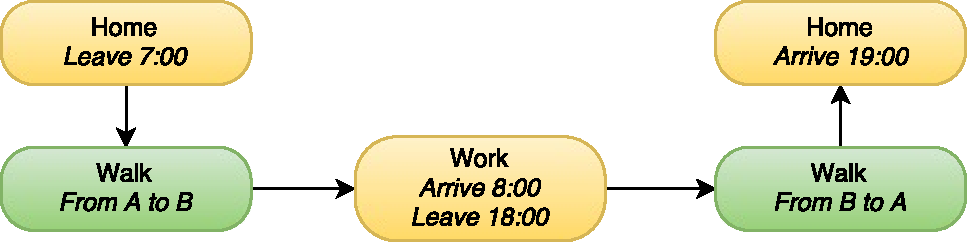
\includegraphics[width=0.8\textwidth]{../simpleplan.pdf}
\label{fig:typical_plan}
\caption{A typical agent plan in MATSim}
\end{figure}

The network, on which the simulation is taking place, is decribed through nodes
 and connecting links. These are described by a specific capacity which tells the
 simulation how many vehicles are able to pass the link within a certain time
 frame, while the the length and an average link speed determine how fast vehicles
 will travel to the next node.

 The whole MATSim simulation is done time-step by time-step. In a single simulation step (usually 1 second)
 the agents that are currently in an activity don't need to be taken into account unless their scheduled
 activity end is reached. The other agents, which are currently on a leg, are simulated in a
 dedicated traffic network simulation. This simulation moves the agents according
 to the capacity and current congestion from the start node to the end node of the
 respective links. Traffic is not simulated on a micro-level (i.e. the vehicles
 don't have distinct positions along the link) in order to increase the simulation
 speed.

The congestion on the traffic network is therefore emerging from the single travel
plans of all the agents. If there are too many agents which try to use one route
at the same time, the overall congestion will increase.

All steps described above, i.e. the simulation of acitivities and legs during
a whole day, are summarized as the ``Mobility Simulation'' or, in short, Mobsim
of the MATSim framework.

In order to simulate dynamic agents, which are not statically residing in a
fixed-timed activity or a predefined leg route, quite significant changes need
to be made and some of the computational advantages of the simulation approach
need to be partly circumvented. This, however, mainly addresses implementational
details and will be discussed later throughout the thesis in chapter \ref{sec:dynagent}.

\section{Utility-based scoring}

As pointed out in the last section, individual travel decisions might lead to
waiting times on the network, which then can also lead to late arrivals at the
designated activity locations, which usually would be disadvantageous in the real
world. Therefore, it might be beneficial for an agent to reconsider the time and
route choices that had been made for the current day, just as a real person
would do.

In order to ``know'' whether a plan worked out well or was disadvantageous, the
single elements need to be weighed and quantified. This is done using the Charypar-Nagel
scoring function \cite{Horni2015}:

\begin{equation}
S_{plan} = \sum_{q=0}^{N-1} S_{act,q} + \sum_{q=0}^{N-1} S_{trav,mode(q)}
\end{equation}

Basically, it combines the marginal utilities of all activities ($S_{act,q}$) ranging
over the $N$ activities in a plan and the marginal utilities for all the legs in
between.

The marginal utility for the activities, among other factors, depends on how long
the activity has been performed, whether the agent needed to wait to start it (due
to an early arrival) or whether it was forced to leave early. For more details
the complete computation is shown in \cite{Horni2015}.

For the scope of this thesis the travel utility is more interesting. A basic version
for a single leg $q$ can look as follows:

\begin{equation}\begin{aligned}
S_{trav,mode(q)} &= C_{mode(q)} \\ &+ \beta_{trav,mode(q)} \cdot t_{trav,q} \\
&+ \gamma_{d,mode(q)} \cdot \beta_{m} \cdot d_{trav,q}
\end{aligned}\end{equation}

The first term, $\mathbf{C_{mode(q)}}$, describes a constant (dis)utility for the
choosing a certain mode for the leg. It can be interpreted as how ``favorable''
a certain mode is and is generally negative.\\

The parameter $\mathbf{\beta_{trav,mode(q)}}$ is the marginal utility of traveling,
which is multiplied by the time spent on the leg $t_{trav,q}$. It signifies how
favorable it is to spend time on such a leg, i.e. the longest one needs to stay
in a car or in the public transport, the larger the disutility gets (and therefore
the parameter is usually negative). Values which are absolutely bigger therefore
stand for travel modes where time is spent less useful or comfortably.\\

The third element involves the (positive) marginal utility of money $\mathbf{\beta_{m}}$,
which is an universal simulation parameter and describes how the utility of money can
be weighed against e.g. time.
It is multiplied with the (negative) monetary distance rate
$\mathbf{\gamma_{d,mode(q)}}$, which states, to how much disutility per spanned
distance the leg will lead. This parameter is useful for imposing distance-based
fares in a certain transport mode and thus making it monetarily attractive or
unattractive compared to other ways of traveling.\\

Beyond these parameters, which are usually used by all travel modes, there are
a number of additions, e.g. for public transport, or yet generally unused options, such
as a direct marginal utility of distance travelled.

For the purpose of simulation autonomous taxi services, two additions are made:

\begin{equation}\begin{aligned}
S_{av} &= C + \beta_{trav} \cdot t_{trav} + \gamma_d \cdot \beta_m \cdot d_{trav}\\
&+ \beta_{wait} \cdot t_{wait} + f_m(d_{trav},t_{trav})
\end{aligned}\end{equation}

Here, $\mathbf{\beta_{wait}}$ is the marginal utility of waiting time, quantifying
how disadvantageous it is to wait for a taxi to arrive. Furthermore the function
$f_m(\cdot)$ is a placeholder for any pricing strategy that might be tested. The
implementation will allow for an easy modification of this function.

All these utility computations are done after all agents have been simulated for
a whole day (in fact, usually 30h are used). This step in the MATSim framework is
simply called the ``scoring'' phase.

\section{Evolutionary replanning}

The last step in order to make all the agents ``learn'' more optimal plans which
make sure that they arrive on time at the activity locations and avoid congestion
is to make them replan their day. This is done using an evolutionary algorithm in
the following way:

Usually an agent will start out with one quite random plan, go through it during
one whole day and then get a score for it. Afterwards, in some iterations, this
plan is copied and modified slightly. Those modifications can happen with respect
to start and end times of activities, mode choices for certain legs, etc. So after
one iteration the agent might already have two plans to choose from.

Before the next day starts, one of the available plans is selected due to a certain
strategy. The standard approach is to do a multinomial selection with respect to
the previously obtained plan scores. So one after another plans, will be created,
scored, modified, rescored and so on. Because of the selection process, which
favors high scores, better and better choices will be made.

However, this is done for each and every agent, so while improving the performance
of one agent's plans, this might effect the performance of other agents negatively,
which is especially true if one thinks about the example of highly congested roads
due to too many agents choosing the same route. Finally though, the algorithm reach
at a quasi-equilibirum, which in MATSim is usually refered to as the ``relaxed
state'', in which the average score of the used plans stabilizes within a
reasonable variance.

Each ``day'' that is simulated in this manner is usually called an ``iteration''
of the simulation. It is common to divide these iterations into two parts. The
first one is the ``innovation phase'', where plans have a certain probability to
be modified, while in the second phase innovation is turned off. This means that
the agent will only choose among the present plans in his repertoire (usually
around 5) and rescore them again and again, until the most favorable is selected.

All of the above is known as the ``replanning'' in MATSim. Putting everything
together, a whole cycle in a MATSim simulation can be seen in figure \ref{fig:matsimcycle}. Since the
final traffic situation evolves from the evolutionary choice in the replaning and
selection, as well as from the emergent congestion in the Mobsim, this whole
cycle is usually referred to as a ``co-evolutionary'' algorithm.

Figure \ref{fig:scorestats} shows a typical progression of the population-wide
score in a MATSim simulation. What one can see there is an average over the worst
or best plans of each agent, additionally the averaged average score of all the
plans that the agents own is displayed. Finally one can see the average of all
the plans that have been executed by the agents in a particular iteration.

The first phase until iteration 100 is the innovation phase, where time and mode
choices can be done, while at iteration 100 it is turned off. There, because now
the best plans must adapt to the overall situation, they are loosing in value,
while the worst scored plans are dropped are likely to be discarded. Finally,
a quite stable population-wide relaxed state is reached.

\begin{figure}
\centering
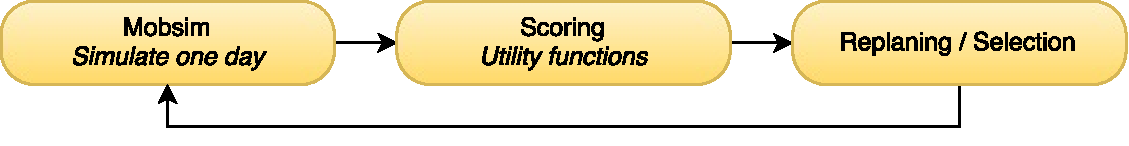
\includegraphics[width=1.0\textwidth]{../matsimcycle.pdf}
\label{fig:matsimcycle}
\caption{The basic co-evolutionary algorithm of MATSim, showing the three main
stages: Mobsim, Scoring and Replanning/Selection}
\end{figure}

\begin{figure}
\centering
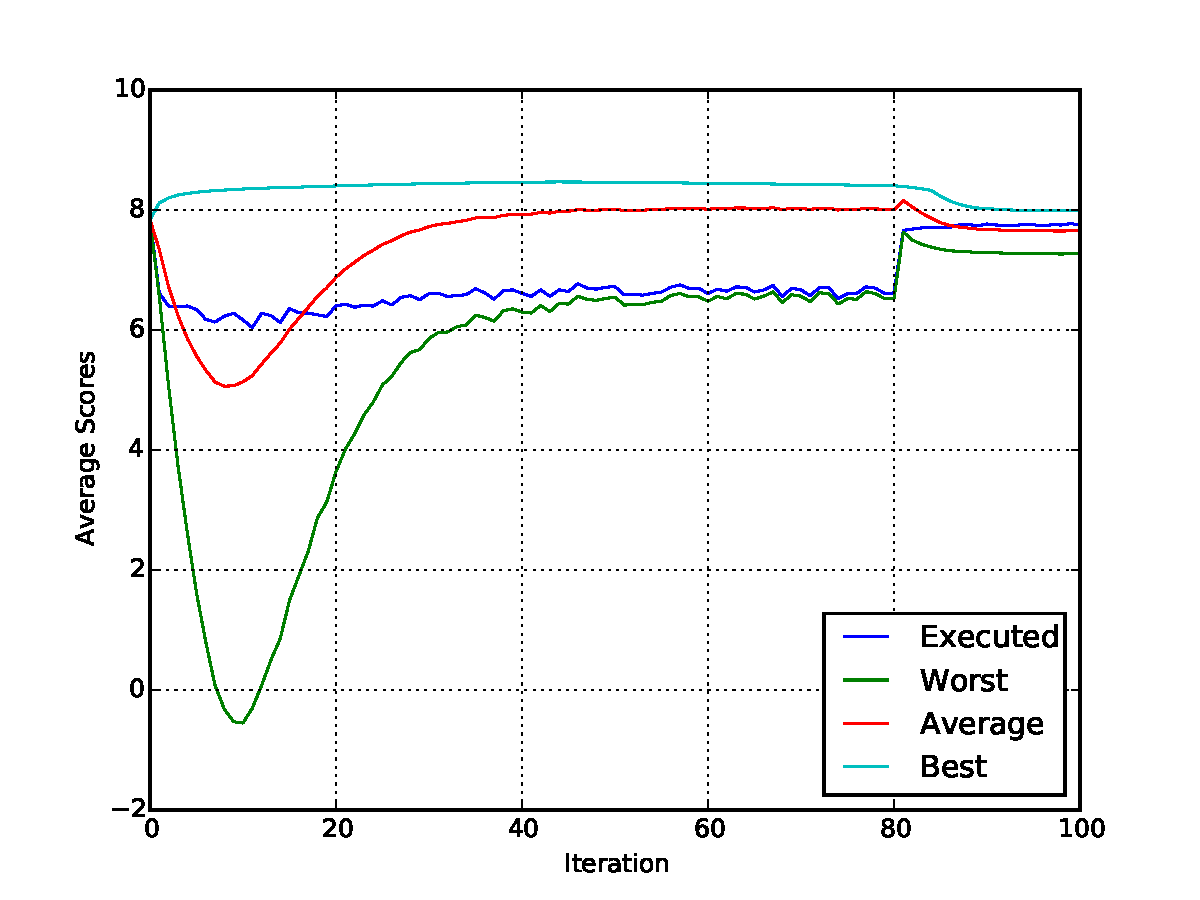
\includegraphics[width=1.0\textwidth]{../scorestats.pdf}
\label{fig:scorestats}
\caption{Typical progression of the agent scores throughout a MATSim simulation.
``Worst'' means that the plans with the worst scores from all the agents are taken
and averaged, the same applies for the other graphs.}
\end{figure}
